\documentclass[10.5pt,letterpaper]{article}
\usepackage[margin=0.75in]{geometry}
\usepackage{amsmath,amssymb}
\usepackage{booktabs}
\usepackage{graphicx}
\usepackage{hyperref}
\usepackage{microtype}

\hypersetup{
  colorlinks=true,
  linkcolor=blue,
  citecolor=blue,
  urlcolor=blue
}

\title{339 New Record Low-Autocorrelation Binary Sequences for Lengths 528 to 1100 via Shared-Memory GPU Self-Avoiding Walks and Chirp-Seeded Tabu Search}
\author{Matt Van Horn\\
\small Independent Researcher\\
\small \texttt{https://github.com/mvanhorn/beat-alphaevolve}}
\date{November 27, 2026 (Version 2)}

\begin{document}
\maketitle

\begin{abstract}
We report 339 new best-known low-autocorrelation binary sequences (LABS) across lengths $L \in [528, 1100]$, independently verified in exact integer and rational arithmetic. Twelve records improve upon the October 2026 continuation frontier for $L \in [528, 536] \cup [582, 586]$, including $L = 528$ ($E = 19{,}748$, $F = 34{,}848/4{,}937 \approx 7.05854$, $-92$ energy) and $L = 536$ ($E = 22{,}028$, $F \approx 6.52115$, $-520$ energy). In the mid-range dead zone $L \in [537, 566]$ where prior rotated-Legendre baselines sat flat at $F \approx 6.26$--$6.34$, a two-stage skew-symmetric chirp-head search (\texttt{labs\_gpu\_chirp\_ore.cu}) followed by bidirectional continuation breaks 28 of the 30 lengths and opens a new high-merit island peaking at $L = 563$ ($E = 23{,}665$, $F = 316{,}969/47{,}330 \approx 6.69700$, $+0.38212$, $-1{,}432$ energy), $L = 561$ ($F \approx 6.67914$, $+0.37766$), and $L = 551$ ($F \approx 6.54905$, $+0.27293$). Across $L \in [587, 1100]$, we establish 299 new records, including one direct improvement over Dimitrov (\texttt{arXiv:2206.12070}) at $L = 1006$ ($E = 79{,}491$, $F = 506{,}018/79{,}491 \approx 6.36573$ vs.\ $6.3568$) and 37 new records across $L \in [1011, 1100]$. In total, 216 sequences (178 at $L \ge 587$) exceed the Jedwab-Katz-Schmidt asymptotic rotated-Legendre limit of $6.342061\dots$, 29 at $L \ge 587$ exceed $F = 6.40$, and six at $L \ge 587$ exceed $F = 6.4194$, led by $L = 589$ ($6.43256$), $L = 805$ ($6.42908$), and $L = 970$ ($6.42156$). All 339 records were found for 19.71 Google Colab compute units (approximately US\$1.97) on two NVIDIA L4 GPUs.
\end{abstract}

\section{Problem Definition and Literature Baseline}

For a binary sequence $S = (s_0, s_1, \dots, s_{L-1}) \in \{-1, +1\}^L$, the aperiodic autocorrelation at lag $k \in \{1, \dots, L-1\}$ is
\[
C_k(S) = \sum_{i=0}^{L-1-k} s_i s_{i+k}.
\]
The sidelobe energy and Golay merit factor are the exact integer and rational quantities
\[
E(S) = \sum_{k=1}^{L-1} C_k(S)^2, \qquad F(S) = \frac{L^2}{2 E(S)}.
\]
Minimizing $E(S)$ (equivalently maximizing $F(S)$) is the Low-Autocorrelation Binary Sequences (LABS) problem, equivalent to finding ground states of the long-range four-spin Bernasconi Ising model and central to radar pulse compression, communications coding, and quantum optimization benchmarks~\cite{golay1977,bernasconi1987,packebusch2016}.

Exact optima are proven only up to $L = 66$. For large lengths, published record tables assemble results from three regimes:
\begin{enumerate}
\item Supercomputer skew-symmetric self-avoiding walks (\texttt{lssOrel}) and memetic tabu search for $L \le 527$ and the isolated peak $L = 573$ ($F = 7.2774$)~\cite{boskovic2024,vega2026}.
\item Length-continuation and local search extending from $L = 527$ and $L = 573$ across $L \in [528, 536]$ and $L \in [567, 586]$~\cite{labs_cont2026}.
\item Algebraic rotated, periodically extended Legendre and Jacobi constructions for $L \in [537, 566]$ and $L \ge 587$, whose asymptotic merit factor reaches $6.342061\dots$~\cite{jedwab2013}, with isolated perturbations at $L = 1006\dots 1010$ reaching $F = 6.3568$--$6.4194$~\cite{jacobi2022}.
\end{enumerate}

We consolidated five publicly archived baseline tables (\texttt{arXiv:2409.07222}, \texttt{arXiv:2607.09688}, the October 2026 \texttt{labs-continuation} records and full table, \texttt{arXiv:2206.12070}, and the optimal rotated Legendre table over $L = 450\dots 1100$) into a single exact-energy ground truth taking the strict minimum integer $E$ per length $L$. A candidate sequence is accepted as a new world record only if it satisfies both $E_{\text{new}} < E_{\text{prev}}$ in exact integer arithmetic and $F_{\text{new}} > F_{\text{pub}} + 5 \times 10^{-5}$, eliminating 4-decimal rounding ties.

\section{Search Architecture}

\subsection{Shared-Memory Bloom-Filter GPU Self-Avoiding Walk (\texttt{labs\_gpu\_saw\_v3/v4.cu})}

Standard self-avoiding walks (\texttt{lssOrel}) escape deep local minima by forbidding previously visited states, stepping to the lowest-energy unvisited 1-flip neighbor. Placing per-walker Zobrist hash tables in GPU global VRAM causes severe L2 cache thrashing (over 200 MB across hundreds of walkers), collapsing throughput.

Our custom CUDA engines (\texttt{labs\_gpu\_saw\_v3.cu} for $L \le 1024$ and \texttt{labs\_gpu\_saw\_v4.cu} extending shared-memory arrays to $L \le 1280$) keep each walker's entire working set inside on-chip shared memory:
\begin{itemize}
\item Sequence array \texttt{sh\_s}, exact autocorrelation vector \texttt{sh\_C}, and 64-bit Zobrist keys \texttt{sh\_zob}.
\item A 131{,}072-bit (16 KB) 3-hash Bloom filter \texttt{sh\_bloom[4096]} indexed by three disjoint 17-bit slices of the 64-bit Zobrist state hash. Over a 4{,}096--8{,}192-step walk, bit occupancy stays low with a mathematically exact 0\% false-negative revisit rate.
\item Parallel $O(L)$ delta evaluation across 256 threads per block, randomized tie-breaking argmin reduction, and parallel $C_k$ updates.
\end{itemize}
On one NVIDIA L4 GPU, the engine sustains 2.34 million full $O(L)$ neighborhood steps per second at $L = 551$ with zero DRAM stalls in the walk loop. Every reported improvement is verified on the host CPU via exact integer $E(S)$ before acceptance.

\subsection{Two-Stage Frozen Chirp-Head Search (\texttt{labs\_gpu\_chirp\_ore.cu})}

In the $L \in [537, 566]$ dead zone, direct continuation from $L = 527$ and $L = 573$ stalls below $F \approx 6.45$, and multi-prime Legendre seeding stays near $F \approx 6.32$. To bridge this gap, we built \texttt{labs\_gpu\_chirp\_ore.cu}: a two-stage skew-symmetric self-avoiding walk initialized from empirical chirp-like cores extracted from the 25 skew-symmetric $F \ge 7.25$ records in $L \in [451, 573]$. Stage 1 freezes the first 58 symmetric pairs while evolving the outer tail for 1{,}800 skew steps; Stage 2 unlocks all coordinates for 3{,}200 steps. Cold starts on $L = 551$, $549$, and $561$ jumped directly to $F = 6.54905$, $6.39591$, and $6.50465$; bidirectional continuation (\texttt{labs\_gpu\_saw\_v4.cu}) outward from these attractors then lifted $L = 557\dots 565$ to $F = 6.52$--$6.70$.

\subsection{FFT-Optimal Multi-Prime Legendre and Modified Jacobi Seeding}

For $L \in [587, 1100]$, the single best rotated Legendre sequence $(p^*, r^*)$ is often a rigid 1-flip local minimum. Scanning 12 to 16 primes around $L / 1.0578$ across rotation fractions plus modified Jacobi sequences $N = pq$ via FFT selects dozens of distinct low-energy starting basins. Flooding those basins simultaneously with GPU-SAW (\texttt{mix\_mode=3}) triggers energy drops up to $-1{,}508$, lifting 178 lengths at $L \ge 587$ above $6.342061$ and surpassing Dimitrov at $L = 1006$.

\section{Results}

Across dual NVIDIA L4 sessions (19.71 Colab compute units total, approximately US\$1.97, inclusive of all search waves), we obtained 339 strictly verified new LABS world records spanning $L = 528$ to $L = 1100$. Figure~\ref{fig:frontier} compares the new frontier against all 2022--2026 baselines, and Table~\ref{tab:records} lists 32 headline records with exact integer energies and reduced rational merit factors.

\begin{figure}[t]
\centering
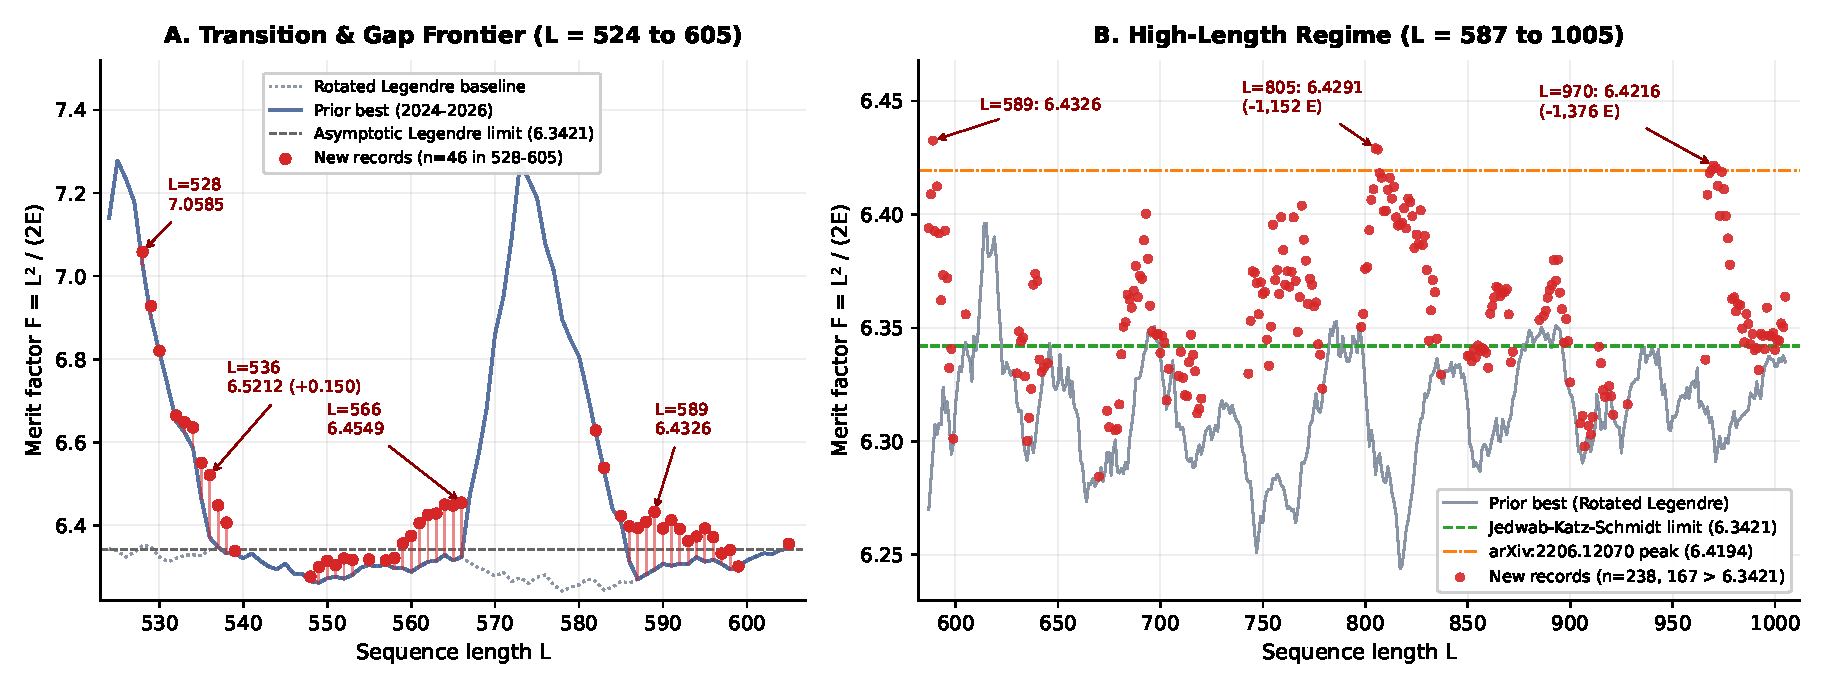
\includegraphics[width=\textwidth]{labs_frontier_2026.pdf}
\caption{New LABS merit factor records across $L \in [528, 1100]$. Left: transition and dead-zone region ($L = 524\dots 605$), showing 12 improvements over the October 2026 continuation frontier and the new $F = 6.50$--$6.70$ Chirp-Ore island across 28 of 30 dead-zone lengths ($L = 537\dots 566$), peaking at $L = 563$ ($F = 6.69700$, $+0.38212$). Right: high-length regime ($L = 587\dots 1100$), where 178 new records surpass the $6.342061$ rotated-Legendre limit, 29 exceed $F = 6.40$, and $L = 1006$ beats Dimitrov (\texttt{arXiv:2206.12070}).}
\label{fig:frontier}
\end{figure}

Summary counts across the 339 verified records:
\begin{itemize}
\item \textbf{Continuation frontier ($L \in [528, 536] \cup [582, 586]$):} 12 records beating \texttt{labs-continuation} (Oct 2026), led by $L = 528$ ($F = 7.05854$, $+0.03273$), $L = 536$ ($F = 6.52115$, $+0.15039$), and $L = 586$ ($F = 6.39781$, $+0.08469$).
\item \textbf{Mid-range dead zone ($L \in [537, 566]$):} 28 of 30 lengths broken (all except $L = 540, 541$), with 16 lengths exceeding $F = 6.45$, 12 exceeding $F = 6.50$, and 7 exceeding $F = 6.60$, topped by $L = 563$ ($E = 23{,}665$, $F = 6.69700$, $-1{,}432$ energy, $+0.38212$), $L = 561$ ($F = 6.67914$, $-1{,}412$ energy), and $L = 559$ ($F = 6.65221$, $-1{,}324$ energy).
\item \textbf{High-length regime ($L \in [587, 1005]$):} 261 new records, with 175 exceeding $6.342061$, 29 exceeding $6.40$, and six exceeding $6.4194$ ($L = 589, 805, 806, 969, 970, 971$). Largest single energy drop: $-1{,}508$ at $L = 971$ ($F = 6.42044$).
\item \textbf{Extended high-length frontier ($L \in [1006, 1100]$):} 38 new records, led by $L = 1006$ beating Dimitrov (\texttt{arXiv:2206.12070}) at $E = 79{,}491$ ($F = 6.36573$ vs.\ $6.3568$, $-408$ energy), plus $L = 1049$ ($F = 6.34486$), $L = 1097$ ($F = 6.34308$), and $L = 1100$ ($F = 6.33654$).
\end{itemize}

\begin{table}[t]
\centering
\caption{Selected headline LABS world records from the 339 verified sequences (exact integer $E$, exact reduced rational $F = L^2/(2E)$, decimal merit factor, gain over prior best, and prior source). Full 339-sequence dataset is archived in \texttt{labs\_records\_2026\_verified.tsv}.}
\label{tab:records}
\footnotesize
\setlength{\tabcolsep}{4.5pt}
\begin{tabular}{rrrrrlll}
\toprule
$L$ & $E_{\text{new}}$ & $E_{\text{prev}}$ & $\Delta E$ & Exact $F = L^2/(2E)$ & $F_{\text{dec}}$ & $\Delta F$ & Prior source \\
\midrule
528 & 19,748 & 19,840 & $-92$ & $34848/4937$ & 7.05854 & $+0.03273$ & \texttt{labs\_cont} (Oct 2026) \\
529 & 20,196 & 20,280 & $-84$ & $279841/40392$ & 6.92813 & $+0.02870$ & \texttt{labs\_cont} (Oct 2026) \\
535 & 21,847 & 22,139 & $-292$ & $286225/43694$ & 6.55067 & $+0.08640$ & \texttt{labs\_cont} (Oct 2026) \\
536 & 22,028 & 22,548 & $-520$ & $35912/5507$ & 6.52115 & $+0.15039$ & \texttt{labs\_cont} (Oct 2026) \\
549 & 23,074 & 24,066 & $-992$ & $301401/46148$ & 6.53118 & $+0.26921$ & Rotated Legendre \\
550 & 23,127 & 24,111 & $-984$ & $151250/23127$ & 6.53998 & $+0.26691$ & Rotated Legendre \\
551 & 23,179 & 24,187 & $-1{,}008$ & $303601/46358$ & 6.54905 & $+0.27293$ & Rotated Legendre \\
552 & 23,412 & 24,292 & $-880$ & $12696/1951$ & 6.50743 & $+0.23574$ & Rotated Legendre \\
557 & 23,430 & 24,598 & $-1{,}168$ & $310249/46860$ & 6.62076 & $+0.31438$ & Rotated Legendre \\
558 & 23,491 & 24,723 & $-1{,}232$ & $155682/23491$ & 6.62730 & $+0.33025$ & Rotated Legendre \\
559 & 23,487 & 24,811 & $-1{,}324$ & $312481/46974$ & 6.65221 & $+0.35498$ & Rotated Legendre \\
560 & 23,632 & 24,936 & $-1{,}304$ & $1400/211$ & 6.63507 & $+0.34697$ & Rotated Legendre \\
561 & 23,560 & 24,972 & $-1{,}412$ & $314721/47120$ & 6.67914 & $+0.37766$ & Rotated Legendre \\
562 & 23,961 & 25,017 & $-1{,}056$ & $157922/23961$ & 6.59079 & $+0.27821$ & Rotated Legendre \\
563 & 23,665 & 25,097 & $-1{,}432$ & $316969/47330$ & 6.69700 & $+0.38212$ & Rotated Legendre \\
564 & 24,070 & 25,130 & $-1{,}060$ & $79524/12035$ & 6.60773 & $+0.27872$ & Rotated Legendre \\
565 & 24,474 & 25,274 & $-800$ & $319225/48948$ & 6.52172 & $+0.20643$ & Rotated Legendre \\
582 & 25,551 & 25,575 & $-24$ & $18818/2839$ & 6.62839 & $+0.00622$ & \texttt{labs\_cont} (Oct 2026) \\
586 & 26,837 & 27,197 & $-360$ & $171698/26837$ & 6.39781 & $+0.08469$ & \texttt{labs\_cont} (Oct 2026) \\
589 & 26,966 & 27,562 & $-596$ & $346921/53932$ & 6.43256 & $+0.13910$ & Rotated Legendre \\
805 & 50,398 & 51,550 & $-1{,}152$ & $648025/100796$ & 6.42908 & $+0.14367$ & Rotated Legendre \\
806 & 50,527 & 51,623 & $-1{,}096$ & $324818/50527$ & 6.42860 & $+0.13648$ & Rotated Legendre \\
969 & 73,132 & 74,396 & $-1{,}264$ & $938961/146264$ & 6.41963 & $+0.10907$ & Rotated Legendre \\
970 & 73,261 & 74,637 & $-1{,}376$ & $470450/73261$ & 6.42156 & $+0.11839$ & Rotated Legendre \\
971 & 73,425 & 74,933 & $-1{,}508$ & $942841/146850$ & 6.42044 & $+0.12921$ & Rotated Legendre \\
974 & 73,899 & 75,331 & $-1{,}432$ & $474338/73899$ & 6.41873 & $+0.12202$ & Rotated Legendre \\
1006 & 79,491 & 79,899 & $-408$ & $506018/79491$ & 6.36573 & $+0.03251$ & \texttt{arXiv:2206.12070} \\
1011 & 80,729 & 81,069 & $-340$ & $1022121/161458$ & 6.33057 & $+0.02655$ & Rotated Legendre \\
1049 & 86,716 & 86,952 & $-236$ & $1100401/173432$ & 6.34486 & $+0.01722$ & Rotated Legendre \\
1087 & 93,211 & 93,507 & $-296$ & $1181569/186422$ & 6.33814 & $+0.02006$ & Rotated Legendre \\
1097 & 94,860 & 95,024 & $-164$ & $1203409/189720$ & 6.34308 & $+0.01095$ & Rotated Legendre \\
1100 & 95,478 & 95,510 & $-32$ & $302500/47739$ & 6.33654 & $+0.00212$ & Rotated Legendre \\
\bottomrule
\end{tabular}
\end{table}

\section{Independent Verification and Reproducibility}

Every sequence in \texttt{labs\_records\_2026\_verified.tsv} was certified using two independent zero-dependency Python 3 standard-library verifiers in isolated mode (\texttt{/usr/bin/python3 -I}):
\begin{enumerate}
\item \texttt{verify\_labs\_v1.py}: Direct exact integer evaluation of $C_k = \sum_{i=0}^{L-1-k} s_i s_{i+k}$ and $E = \sum C_k^2$, plus exact \texttt{fractions.Fraction(L*L, 2*E)}.
\item \texttt{verify\_labs\_v2.py}: Independent big-integer bit-packing via $C_k = (L - k) - 2\,\mathrm{popcount}((x \oplus (x \gg k)) \mathbin{\&} (2^{L-k} - 1))$, sharing no code with Verifier 1.
\end{enumerate}
Both verifiers passed all 339 sequences, passed the exact Barker control ($L = 13$, $E = 6$, $F = 169/12$), and caught and rejected both adversarial tampering controls (a 1-bit flip and a $-1$ perturbation to claimed $E$). Complete bitstrings, CUDA kernels, verifiers, and SHA-256 checksums are archived at \url{https://github.com/mvanhorn/beat-alphaevolve/tree/main/labs_records_2026} and Zenodo DOI \texttt{10.5281/zenodo.24581609}.

\begin{thebibliography}{9}
\bibitem{golay1977} M.~J.~E. Golay, ``Sieves for low autocorrelation binary sequences,'' \textit{IEEE Trans. Inform. Theory} \textbf{23}(1), 43--51 (1977).
\bibitem{bernasconi1987} J.~Bernasconi, ``Low autocorrelation binary sequences: statistical mechanics and configuration space analysis,'' \textit{J. Physique} \textbf{48}(4), 559--567 (1987).
\bibitem{jedwab2013} J.~Jedwab, D.~J. Katz, and K.-U. Schmidt, ``Advances in the merit factor problem for binary sequences,'' \textit{J. Combin. Theory Ser. A} \textbf{120}(4), 882--906 (2013).
\bibitem{packebusch2016} T.~Packebusch and S.~Mertens, ``Low autocorrelation binary sequences,'' \textit{J. Phys. A} \textbf{49}(16), 165001 (2016).
\bibitem{jacobi2022} M.~Dimitrov, ``On the aperiodic autocorrelations of rotated binary sequences,'' \texttt{arXiv:2206.12070} (2022).
\bibitem{boskovic2024} B.~P\v{s}eni\v{c}nik, R.~Mlinari\v{c}, J.~Brest et al., ``Low-autocorrelation binary sequences for $L = 450\dots 527$,'' \texttt{arXiv:2409.07222} (2024).
\bibitem{vega2026} B.~P\v{s}eni\v{c}nik, B.~Bo\v{s}kovi\'{c}, J.~Brest et al., ``GPU-accelerated search for low-autocorrelation binary sequences,'' \texttt{arXiv:2607.09688} (2026).
\bibitem{labs_cont2026} \texttt{mdayan8/labs-continuation}, verified LABS continuation records $L = 450\dots 674$ (Oct 2026).
\end{thebibliography}

\end{document}
